\section{HTML5}

Algunas de las nuevas características que incluye la versión más reciente de HTML son los formularios 2.0, que traen controles para seleccionar fechas, colores, números, cajas de texto para correos electrónicos, búsqueda, URL, los métodos PUT y DELETE, entre otros; el tipo de documento previo al inicio de la estructura HTML, nuevas etiquetas, la posibilidad de modificar la codificación de caracteres, entre otros temas que se verán en este documento.


\subsection{Modelos de contenido}

Los \textbf{modelos de contenido} son modelos de etiquetas que responden a una misma función o que tienen un fin determinado, los modelos pueden ir enfocados a la interacción, la organización, inserción, formateo o adición de información de una página o sitio web. Estos modelos suelen contener ciertas etiquetas que responden al fin del mismo.

Anteriormente, habíamos mencionado que HTML tenía etiquetas Block-Level e Inline, donde la segunda suele pertenecer a la primera (revisar la sección \textbf{Tipos de elementos}), en esta versión del lenguaje, se agregan siete modelos nuevos:
\begin{enumerate}
    \item Metadata: establece información adicional o comportamiento al resto del contenido de la página o sitio. Podemos encontrar las siguientes etiquetas en este modelo: \textbf{base}, \textbf{link}, \textbf{meta}, \textbf{noscript}, \textbf{script}, \textbf{style}, \textbf{title}.
    \item Embedded: contenido que es importado a la estructura o contenido de la página o sitio. Podemos encontrar las siguientes etiquetas en este modelo: \textbf{audio}, \textbf{video}, \textbf{canvas}, \textbf{iframe}, \textbf{img}, \textbf{math}, \textbf{object}, \textbf{svg}.
    \item Interactive: contenido hecho para que el usuario interactue con él. Podemos encontrar las siguientes etiquetas en este modelo: \textbf{a}, \textbf{audio}, \textbf{video}, \textbf{button}, \textbf{details}, \textbf{embed}, \textbf{iframe}, \textbf{img}, \textbf{input}, \textbf{label}, \textbf{object}, \textbf{select}, \textbf{textarea}.
    \item Heading: establece cabeceras o secciones en el documento. Podemos encontrar las siguientes etiquetas en este modelo: \textbf{h1} a \textbf{h6} y \textbf{hgroup}.
    \item Phrasing: es un modelo para formatear contenido, posee varias etiquetas compartidas con HTML4: \textbf{img}, \textbf{span}, \textbf{strong}, \textbf{label}, \textbf{br/}, \textbf{small}, \textbf{sub} y más.
    \item Flow: contiene la mayoría de las etiquetas que serán utilizadas en la estructura, flujo o funcionamiento del documento. Se puede decir que este modelo incluye la mayoría del resto.
    \item Sectioning: establece el objetivo de las secciones, contenido, navegación o pies de páginas. Podemos encontrar las siguientes etiquetas en este modelo: \textbf{article}, \textbf{aside}, \textbf{nav}, \textbf{section}.
\end{enumerate}

La \textit{Figura \ref{fig: 12}} nos muestra un diagrama de como se relacionan estos modelos:
\begin{figure}[H]
    \centering
    \caption{Relación de los modelos de contenido HTML5}
    \label{fig: 12}
    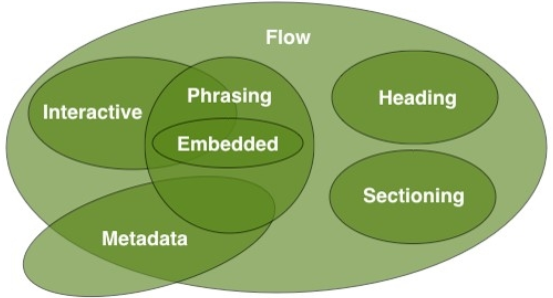
\includegraphics[width=9cm]{ss_html/modelos.png}
\end{figure}

Ojo, no es como que tengamos que escoger un modelo para desarrollar nuestro proyecto, simplemente son contenedores de etiquetas que tienen un fin específico.


\subsection{Estructura de páginas HTML5}

La estructura básica o más simple de un sitio web moderno HTML5 se aprecia en la \textit{Figura \ref{fig: 13}} (no es necesario que se agreguen todas las secciones de esta estructura):
\begin{figure}[H]
    \centering
    \caption{Estructura básica de un sitio web HTML5}
    \label{fig: 13}
    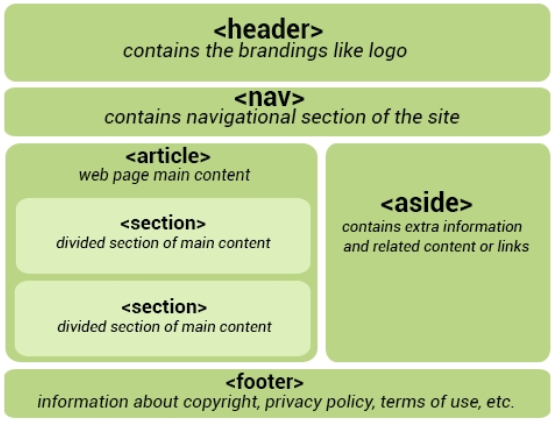
\includegraphics[width=9cm]{ss_html/estructura basica_html5.png}
\end{figure}


\subsubsection{headers, nav y footer}
\hspace{0.55cm}La etiqueta \textbf{header} es la cabecera del sitio, donde está el logo del sitio o información más importante del sitio, si queríamos crear un \textit{header} con HTML4, debíamos utilizar un contenedor \textbf{div}:
\begin{center}
    \textit{$<$div id="header"$>$}
\end{center}

Con HTML5, poseemos la etiqueta \textbf{header} que vuelve más fácil esta tarea:
\begin{lstlisting}
    <!-- Cabecera del sitio. -->
    <header>
	<h1>Nombre y logo del sitio</h1>
    </header>
    <!-- Resto del sitio. -->
    <h3>Esto es el cuerpo del sitio</h3>
    <h3>Esto es el cuerpo del sitio</h3>
    <h3>Esto es el cuerpo del sitio</h3>
\end{lstlisting}

La etiqueta \textbf{nav} es un menú horizontal que te permite navegar a lo largo de todo el sitio web, por lo que \textit{nav} está constituido de enlaces:
\begin{lstlisting}
    <!-- Cabecera del sitio. -->
    <header>
        <h1>Nombre y logo del sitio</h1>
    </header>
    <!-- Barra de navegación del sitio. -->
    <nav>
        <ul>
            <li><a href="#">Home</a></li>
            <li><a href="#">Servicios</a></li>
            <li><a href="#">Acerca de nosotros</a></li>
            <li><a href="#">Organigrama</a></li>
        </ul>
    </nav>
    <!-- Resto del sitio. -->
    <h3>Esto es el cuerpo del sitio</h3>
    <h3>Esto es el cuerpo del sitio</h3>
    <h3>Esto es el cuerpo del sitio</h3>
\end{lstlisting}


La etiqueta \textbf{footer} es el pie de página del sitio o página, nos permite poner información hasta abajo de la página: este tipo de información suele ser la información de contacto, política de privacidad, redes sociales, términos de uso, información de Copyright, documentos relacionados, mapa del sitio, etc:
\begin{lstlisting}
    <!-- Cabecera del sitio. -->
    <header>
        <h1>Nombre y logo del sitio</h1>
    </header>
    <!-- Barra de navegación del sitio. -->
    <nav>
        <ul>
            <li><a href="#">Home</a></li>
            <li><a href="#">Servicios</a></li>
            <li><a href="#">Acerca de nosotros</a></li>
            <li><a href="#">Organigrama</a></li>
        </ul>
    </nav>
    <!-- Cuerpo del sitio. -->
    <h3>Esto es el cuerpo del sitio</h3>
    <h3>Esto es el cuerpo del sitio</h3>
    <h3>Esto es el cuerpo del sitio</h3>
    <!-- Pie del sitio. -->
    <footer>
        <h3>Mapa del sitio/h3>
    </footer>
\end{lstlisting}

La \textit{Figura \ref{fig: 14}} muestra el resultado de los dos ejemplos anteriores:
\begin{figure}[H]
    \centering
    \caption{Ejemplo de header y footer}
    \label{fig: 14}
    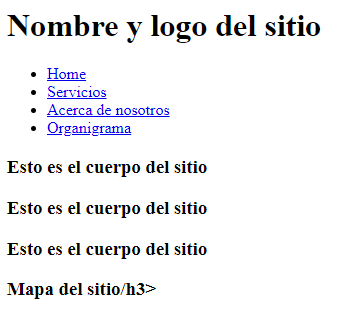
\includegraphics[width=7cm]{ss_html/header_footer.png}
\end{figure}

\textit{Nota}: el buscador ya tiene definido la información de la cabecera, menú de navegación y pie de página, aunque visualmente no parezca nada relevante.


\subsubsection{article, section y aside}

La etiqueta \textbf{article} representa un contenedor para un artículo, foro, post, revista, artículo de periódico, entrada de blog, un comentario, un \textit{widget} o \textit{gadget} interactivo u otro elemento independiente del contenido del sitio, las etiquetas \textit{article} pueden ser anidadas unas dentro de otras, y estos contenedores deben ser independiente al resto del contenido de la página o sitio web. Veamos el siguiente ejemplo:
\begin{lstlisting}
    <article>
        <article>
            <h2>Nombre del artículo</h2>
            <h1>Autor</h1>
        </article>
        <article>
            <h4>Fecha de publicación</h4>
            <h4>Sitio de publicación</h4>
        </article>
        <article>
            <p>Contenido del artículo</p>
        </article>
    </article>
\end{lstlisting}

Anidamos etiquetas \textit{article} dentro de una etiqueta mayor \textit{article}, esto con el fin de que cada etiqueta anidada sea un dato o sección propiamente de un artículo que se esté insertando al documento HTML.

La etiqueta \textbf{section} es un contenedor para diversas etiquetas HTML, estas etiquetas contenidas deben tener algo en común, y es que deben pertenecer a una sección de la página o sitio web; algunas etiquetas que pueden ser utilizadas en las secciones son: \textbf{h1-h6}, \textbf{p}, otra etiqueta \textbf{section} o \textbf{article}. Veamos el siguiente ejemplo:
\begin{lstlisting}
    <article>
        <section>
            <h2>Nombre del artículo</h2>
            <h1>Autor</h1>
        </section>
        <section>
            <h4>Fecha de publicación</h4>
            <h4>Sitio de publicación</h4>
        </section>
        <section>
            <p>Contenido del artículo</p>
        </section>
    </article>
\end{lstlisting}

Se sustituyen los \textit{articles} anidados por \textit{sections}. La diferencia entre article y section es que, article va enfocado contener contenido independiente del sitio web, mientras que section puede contener otros artículos o secciones del propio sitio web.

La etiqueta \textbf{aside} representa contenido relacionado a otro contenido, pudiendo ser este de una etiqueta \textit{article}, de un \textit{section} o del propio sitio web. Veamos un ejemplo:
\begin{lstlisting}
    <article>
        <article>
            <h2>Nombre del artículo</h2>
            <h1>Autor</h1>
        </article>
        <article>
            <h4>Fecha de publicación</h4>
            <h4>Sitio de publicación</h4>
        </article>
        <article>
            <p>Contenido del artículo</p>
        </article>
        <aside>
            <a href="#">Vea estos otros artículos similares</a>
        </aside>
    </article>
\end{lstlisting}

Si copia algunos de los ejemplos anteriores y lo ejecuta en el navegador de su preferencia, verá un sitio bastante sencillo ni diseño particular, pero para el buscador, la existencia de una etiqueta \textit{article}, \textit{section} o \textit{aside} le permitirá una estructuración determinada del sitio.


\subsubsection{\textit{div}, \textit{class} e \textit{id} vs la estructura HTML5}

Veamos sus diferencias:
\begin{itemize}
    \item \textbf{div, class e id}: contenedores de uso muy general, utilizados para contener etiquetas HTML y aplicarles un estilo o evento.
    \item \textbf{article}: contenedor de uso muy específico, para contenido independiente al del sitio o página web.
    \item \textbf{section}: contenedor de uso general, utilizado para contener otras etiquetas \textit{article} o HTML, pero que tengan una relación entre sí.
    \item \textbf{aside}: contenedor para contenido secundario relacionado con respecto a otro.
\end{itemize}


\subsection{La etiqueta audio}

Inserta un archivo de audio a la página o sitio web. Estos son los formatos de audio que aceptan los navegadores más populares:
\begin{itemize}
    \item Internet Explorer: mp3.
    \item Edge: mp3 y wav.
    \item Google Chrome: mp3, wav y ogg.
    \item Firefox: mp3, wav y ogg.
    \item Safari: mp3 y wav.
    \item Opera: wav y ogg.
\end{itemize}

Por este motivo, es que debemos utilizar el siguiente ejemplo para insertar audios a nuestros proyectos:
\begin{lstlisting}
    <!-- Mejor método. -->
    <audio controls>
        <source src="audio1.mp3" type="audio/mpeg">
        <source src="audio2.ogg" type="audio/ogg">
        <source src="audio3.wav" type="audio/wav">
        <!-- Texto a mostrar en caso de que no se pueda reproducir el audio. -->
        Audio no soportado por el buscador.
    </audio>

    <!-- Alternativa. -->
    <audio src="audio1.mp3" controls>
        <!-- Texto a mostrar en caso de que no se pueda reproducir el audio. -->
        Audio no soportado por el buscador.
    </audio>
\end{lstlisting}

El mejor método es denominado así porque el buscador reproduce el audio con el formato que primero reconozca, si no reconoce uno inmediatamente, pasa al siguiente, así sucesivamente; el otro método está limitado a únicamente un audio. Veamos sus atributos:
\begin{itemize}
    \item \textbf{src}: es el archivo a reproducir.
    \item \textbf{autoplay}: reproduce el audio apenas cargue el sitio.
    \item \textbf{loop}: repite el audio indefinidamente.
    \item Los últimos dos atributos pueden funcionar o no según el buscador.
\end{itemize}

La \textit{Figura \ref{fig: 15}} muestra el aspecto de un control \textbf{audio} en el buscador Google Chrome (cambia este aspecto entre buscadores):
\begin{figure}[H]
    \centering
    \caption{Aspecto de la etiqueta audio}
    \label{fig: 15}
    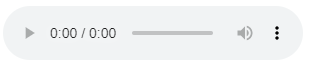
\includegraphics[width=7cm]{ss_html/audio.png}
\end{figure}


\subsection{La etiqueta video}

Inserta un archivo de vídeo a la página o sitio web. Estos son los formatos de audio que aceptan los navegadores más populares:
\begin{itemize}
    \item Internet Explorer: mp4.
    \item Edge: 
    \item Google Chrome: mp4, webm y ogg.
    \item Firefox: mp4, webm y ogg.
    \item Safari: mp4.
    \item Opera: webm y ogg.
\end{itemize}

Posee la misma declaración que las etiquetas \textit{audio}, pero posee atributos muy interesantes:
\begin{lstlisting}
    <!-- Mejor método. -->
    <video controls>
        <source src="video1.mp4" type="video/mp4">
        <source src="video2.ogg" type="video/ogg">
        <source src="video3.webm" type="video/webm">
        <!-- Texto a mostrar en caso de que no se pueda reproducir el video. -->
        Videono soportado por el buscador.
    </video>

    <!-- Alternativa. -->
    <video src="video1.mp4" controls>
        <!-- Texto a mostrar en caso de que no se pueda reproducir el video. -->
        Video no soportado por el buscador.
    </video>
\end{lstlisting}
\begin{itemize}
    \item \textbf{src}: es el archivo a reproducir.
    \item \textbf{autoplay}: reproduce el vídeo apenas cargue el sitio.
    \item \textbf{loop}: repite el vídeo indefinidamente.
    \item \textbf{preload}: carga los datos del vídeo por adelantado.
    \item \textbf{controlList="nodownload"}: evita que el control para descargar el video aparezca.
    \item \textbf{width y height}: dimensionan el vídeo.
    \item \textbf{muted}: reproduce el vídeo sin audio.
    \item \textbf{poster}: asigna una miniatura, cartel o póster al vídeo, previo a su reproducción.
\end{itemize}

La \textit{Figura \ref{fig: 16}} muestra el aspecto de un control \textbf{video} en el buscador Google Chrome (cambia este aspecto entre buscadores):
\begin{figure}[H]
    \centering
    \caption{Aspecto de la etiqueta video}
    \label{fig: 16}
    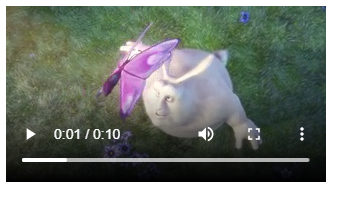
\includegraphics[width=7cm]{ss_html/video.png}
\end{figure}


\subsection{La etiqueta progress}

La etiqueta \textbf{progress} permite insertar una \textbf{Progress Bar} (barra de progreso) en la página o sitio. Sus atributos más importantes son:
\begin{itemize}
    \item \textbf{value}: especifica cuanto de la tarea ha sido completada.
    \item \textbf{min}: especifica el valor inicial de la tarea.
    \item \textbf{max}: especifica el total de trabajo que la tarea debe completar.
\end{itemize}
\begin{center}
    \textit{Estado: $<$progress min="0" max="100" value="35"$>$$<$/progress$>$}
\end{center}

Resultado en Google Chrome (\textit{Figura \ref{fig: 17}}):
\begin{figure}[H]
    \centering
    \caption{Aspecto de la etiqueta progress}
    \label{fig: 17}
    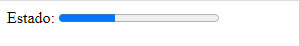
\includegraphics[width=7cm]{ss_html/progress.png}
\end{figure}

Esta etiqueta suele ser utilizada en conjunto con JavaScript, para completar tareas o procesos relacionados con un algo más que las etiquetas de HTML.